% I2C first byte diagram
% Author: Uli Koehler (https://techoverflow.net)
\documentclass[tikz, border=1mm]{standalone}
\usetikzlibrary{positioning, decorations.pathreplacing, arrows.meta}

% Source: https://tex.stackexchange.com/a/24133/45450
\makeatletter
\newcommand*{\textoverline}[1]{$\overline{\hbox{#1}}\m@th$}
\makeatother

\begin{document}
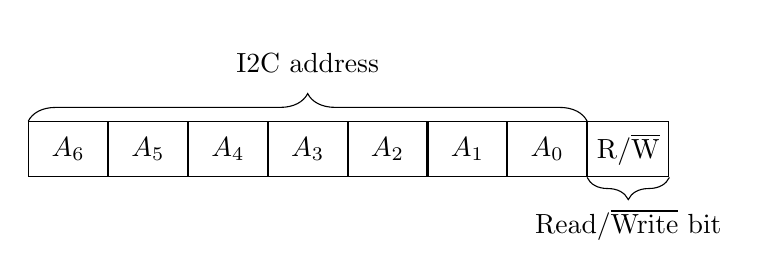
\begin{tikzpicture}
\node (A6) [draw, minimum height=7mm, minimum width=10mm] {$A_6$};
\node (A5) [draw, minimum height=7mm, minimum width=10mm, right=0cm of A6] {$A_5$};
\node (A4) [draw, minimum height=7mm, minimum width=10mm, right=0cm of A5] {$A_4$};
\node (A3) [draw, minimum height=7mm, minimum width=10mm, right=0cm of A4] {$A_3$};
\node (A2) [draw, minimum height=7mm, minimum width=10mm, right=0cm of A3] {$A_2$};
\node (A1) [draw, minimum height=7mm, minimum width=10mm, right=0cm of A2] {$A_1$};
\node (A0) [draw, minimum height=7mm, minimum width=10mm, right=0cm of A1] {$A_0$};
\node (RW) [draw, minimum height=7mm, minimum width=10mm, right=0cm of A0] {R/\textoverline{W}};

\coordinate[above left=0mm of A6] (AddrLeft);
\coordinate[above right=0mm of A0] (AddrRight);

\coordinate[below left=0mm of RW] (RWLeft);
\coordinate[below right=0mm of RW] (RWRight);

\draw[decorate,decoration={brace,amplitude=10pt}, minimum height=9mm]
    (AddrLeft) -- (AddrRight)
    node[anchor=south,midway,above=8pt] {I2C address};

\draw[decorate,decoration={brace,amplitude=8pt}, minimum height=6mm]
    (RWRight) -- (RWLeft)
    node[anchor=north,midway,below=8pt] {Read/\textoverline{Write} bit};

\end{tikzpicture}
\end{document}